\section{Sử dụng Language Model để sửa lỗi kết quả của các mô hình khác}

\subsection{Cơ chế sửa lỗi của Language Model}
\textit{Mô hình ngôn ngữ} (Language Model) thường được sử dụng để sữa lỗi kết quả của những bài toán như Speech to Text hoặc Image to Text.

Xét ví dụ sau:
\begin{itemize}
    \item Câu dự đoán của mô hình nhận diện giọng nói:
    \begin{center}
    The apple and pair salad.
    \end{center}
    \item Câu đúng:
    \begin{center}
    The apple and pear salad.
    \end{center}
\end{itemize}

Trường hợp từ \textit{"pear"} bị dự đoán nhầm thành từ \textit{"pair"} thì mô hình sẽ tính được xác suất của câu \textit{"The apple and pair salad"} sẽ thấp và xác suất của câu \textit{"The apple and pear salad"} sẽ khá cao. Câu hỏi đặt ra là làm sao mô hình tính được xác suất này.

Đó là mô hình sử dụng xác suất có điều kiện để tính được xác suất nêu trên. Tức là đầu tiên sẽ tính xác suất từ \textit{"The"} xuất hiện ở đầu câu, sau đó sẽ tính tiếp trường hợp đầu câu là từ \textit{"The"} và tiếp đó là từ \textit{"apple"} thì xác suất là bao nhiêu. Cứ như thế lần lượt cho \textit{"The apple and"}, \textit{"The apple and pair"} và cuối cùng là khi đã có xác suất của \textit{"The apple and pair"} thì tính tiếp xác suất xuất hiện của từ tiếp đó là \textit{"salad"} là bao nhiêu.

Vậy làm sao để tính được xác suất của từng phần đó. Trước tiên đối với từ \textit{"The"} thì ta sẽ đếm có bao nhiêu câu bắt đầu bằng từ \textit{"The"} trong bộ dữ liệu và từ đó sẽ tính được xác suất của câu bắt đầu bằng từ \textit{"The"}. Tương tự như thế, ta cũng đếm tiếp có bao nhiêu câu bắt đầu bằng từ \textit{"The"} mà tiếp sau đó là từ \textit{"apple"} thì ta cũng tính được xác suất của \textit{"The apple"}. Dựa vào đó ta có thể tính được xác suất cho từng phần đã nêu trên như sau:
\begin{flalign}
\hspace{10mm} &P1 = P(The)& \label{chp7-sec4:eq1} \\
\hspace{10mm} &P2 = P(apple | The) * P1& \label{chp7-sec4:eq2} \\
\hspace{10mm} &P3 = P(and | The\ apple) * P2& \label{chp7-sec4:eq3} \\
\hspace{10mm} &P4 = P(pair | The\ apple\ and) * P3& \label{chp7-sec4:eq4} \\
\hspace{10mm} &P5 = P(salad | The\ apple\ and\ pair) * P4& \label{chp7-sec4:eq5} \\
\hspace{10mm} &P(The\ apple\ and\ pair\ salad) = P5& \label{chp7-sec4:eq6}
\end{flalign}

Sau khi tính được xác suất của câu \textit{"The apple and pair salad"} thì làm sao chúng ta nhận biết được câu này đúng hay sai. Như đã nói ở trên thì sau khi tính được xác suất của câu có từ \textit{"pair"} ta nhận thấy xác suất này khá thấp, so với một \textit{mức} (threshold) đã xác định, nên ta sẽ nghi ngờ rằng câu này chưa đúng. Và cụ thể hơn để xác định từ nào sai thì ta cũng dựa vào xác suất xuất hiện của từng từ được tính toán như trên, đến từ \textit{"pair"} thì xác suất sẽ thấp nên ta có thể nghi ngờ từ \textit{"pair"} là lỗi và sau đó tìm từ thích hợp hơn để thay thế.

Vậy nếu chỉ tính xác suất của cụm từ ngắn hơn trong câu mà có bao gồm từ sai thì có thể nghi ngờ câu đó là câu sai hay không, ví dụ như chỉ tính xác suất của cụm \textit{"and pair"} thì có thể nghi ngờ câu \textit{"The apple and pair salad"} là câu sai hay không.

Việc tính xác suất của chỉ một cụm từ ngắn thì không thể nghi ngờ được câu đang xét có sai hay không bởi xác suất tính được sẽ vẫn đủ cao để không bị nghi ngờ. Vì cụm từ xét tới có thể xuất hiện trong bất cứ ngữ cảnh nào của bộ dữ liệu, tức là cụm đó còn có thể xuất hiện nhiều lần hơn cả cụm đúng mà ta cần sửa lỗi và mức thông tin mà cụm đó cung cấp sẽ thấp bởi vì tính phổ thông của nó lớn, trừ khi cụm xét tới là tên riêng hoặc những cụm từ ít được sử dụng. Vì thế nếu muốn tính đủ xác suất để có thể nghi ngờ từ sai thì chúng ta phải xét cả phần ngữ cảnh trước đó, phần trước đó càng dài thì xác suất sẽ đủ thấp để nghi ngờ từ sai, tức là lượng thông tin được cung cấp sẽ càng nhiều và khả năng phát hiện lỗi sẽ càng cao.

Giả sử bộ dữ liệu gồm 100,000,000 câu, trong đó có:
\begin{itemize}
    \item 25,000,000 câu bắt đầu bằng \textit{"The"}.
    \item 10,000 câu bắt đầu bằng \textit{"The apple"}.
    \item 3,000 câu bắt đầu bằng \textit{"The apple and"}.
    \item 5 câu bắt đầu bằng \textit{"The apple and pair"}.
    \item 250 câu bắt đầu bằng \textit{"The apple and pear"}.
    \item 400 câu bắt đầu bằng \textit{"The apple and strawberry"}.
    \item 1 câu bắt đầu bằng \textit{"The apple and pair salad"}.
    \item 160 câu bắt đầu bằng \textit{"The apple and pear salad"}.
    \item 220 câu bắt đầu bằng \textit{"The apple and strawberry salad"}.
    \item 85,000,000 câu có từ \textit{"and"}.
    \item 13,000 câu có cụm \textit{"and pair"}.
    \item 9,000 câu có cụm \textit{"and pear"}.
    \item 11,000 câu có cụm \textit{"and strawberry"}.
\end{itemize}

Ta có thể tính được các xác suất xuất hiện như sau:
\begin{flalign}
\hspace{10mm} &P(The) = \frac{25,000,000}{100,000,000} = 0.25& \label{chp7-sec4:eq7} \\
\hspace{10mm} &P(The\ apple) = \frac{10,000}{25,000,000}*0.25 = 10^{-4}& \label{chp7-sec4:eq8} \\
\hspace{10mm} &P(The\ apple\ and) = \frac{3,000}{10,000}*10^{-4} = 3*10^{-5}& \label{chp7-sec4:eq9} \\
\hspace{10mm} &P(The\ apple\ and\ pair) = \frac{5}{3,000}*3*10^{-5} = 5*10^{-8}& \label{chp7-sec4:eq10} \\
\hspace{10mm} &P(The\ apple\ and\ pear) = \frac{250}{3,000}*3*10^{-5} = 2.5*10^{-6}& \label{chp7-sec4:eq11} \\
\hspace{10mm} &P(The\ apple\ and\ strawberry) = \frac{400}{3,000}*3*10^{-5} = 4*10^{-6}& \label{chp7-sec4:eq12} \\
\hspace{10mm} &P(The\ apple\ and\ pair\ salad) = \frac{1}{5}*5*10^{-8} = 10^{-8}& \label{chp7-sec4:eq13} \\
\hspace{10mm} &P(The\ apple\ and\ pear\ salad) = \frac{160}{250}*2.5*10^{-6} = 1.6*10^{-6}& \label{chp7-sec4:eq14} \\
\hspace{10mm} &P(The\ apple\ and\ strawberry\ salad) = \frac{220}{400}*4*10^{-6} = 2.2*10^{-6}& \label{chp7-sec4:eq15}
\end{flalign}
Ta có thể thấy xác suất khi xuất hiện từ \textit{"pair"} (công thức \ref{chp7-sec4:eq10}) khá thấp so với \textit{"pear"} (công thức \ref{chp7-sec4:eq11}) và \textit{"strawberry"} (công thức \ref{chp7-sec4:eq12}). Về \textit{mức} (threshold) để xác định từ nghi ngờ là từ sai thì chúng ta có thể giả sử nó sẽ bằng $\frac{1}{100}$ xác suất liền trước (coi như tính cho từ ở vị trí thứ tư). Khi đó:
\begin{equation}
Threshold(The\ apple\ and\ *) = \frac{1}{100} * P(The\ apple\ and) = 3*10^{-7} \label{chp7-sec4:eq16}
\end{equation}
Vì xác suất khi suất hiện của từ \textit{"pair"} thấp hơn threshold đã tính (công thức \ref{chp7-sec4:eq16}) nên ta sẽ nghi ngờ \textit{"pair"} là từ sai. Và ta cũng thấy xác suất của câu \textit{"The\ apple\ and\ pair\ salad"} (công thức \ref{chp7-sec4:eq13}) thấp hơn hẳn \textit{"The\ apple\ and\ pear\ salad"} (công thức \ref{chp7-sec4:eq14}) và \textit{"The\ apple\ and\ strawberry\ salad"} (công thức \ref{chp7-sec4:eq15}).

Với trường hợp tính cho cụm từ ngắn:
\begin{flalign}
\hspace{10mm} &P(and) = \frac{85,000,000}{100,000,000} = 0.85& \label{chp7-sec4:eq17} \\
\hspace{10mm} &P(and\ pair) = \frac{13,000}{85,000,000}*0.85 = 1.3*10^{-4}& \label{chp7-sec4:eq18} \\
\hspace{10mm} &P(and\ pear) = \frac{9,000}{85,000,000}*0.85 = 0.9*10^{-4}& \label{chp7-sec4:eq19} \\
\hspace{10mm} &P(and\ strawberry) = \frac{11,000}{85,000,000}*0.85 = 1.1*10^{-4}& \label{chp7-sec4:eq20}
\end{flalign}
Ta có thể thấy xác suất của \textit{"and\ pair"} (công thức \ref{chp7-sec4:eq18}) còn cao hơn cả \textit{"and\ pear"} (công thức \ref{chp7-sec4:eq19}) và \textit{"and\ strawberry"} (công thức \ref{chp7-sec4:eq20}). Vì thế nên không thể phát hiện \textit{"pair"} là từ sai được bởi thông tin cung cấp bởi \textit{"and\ pair"} còn quá ít.

Trong ví dụ này, \textit{"pear"} và \textit{"strawberry"} đều là những ứng cử viên để thay thế \textit{"pair"}. Tuy nhiên xác suất xuất hiện của \textit{"strawberry"} (công thức \ref{chp7-sec4:eq12}) lớn hơn \textit{"pear"} (công thức \ref{chp7-sec4:eq11}) và xác suất của câu \textit{"The\ apple\ and\ strawberry\ salad"} (công thức \ref{chp7-sec4:eq15}) lớn hơn \textit{"The\ apple\ and\ pear\ salad"} (công thức \ref{chp7-sec4:eq14}), trong khi từ đúng là \textit{"pear"}, vậy làm sao để chọn đúng từ thay thế. Về vấn đề này, khi sửa lỗi, ngoài việc chọn từ có xác suất cao, cần phải quan tâm đến \textit{lĩnh vực} (domain) mà chúng ta đang xử lý.

\subsection{Sử dụng Language Model để sửa lỗi theo lĩnh vực đang xử lý}
Đối với mô hình tổng quát, khi sửa lỗi thì mô hình thường sẽ gợi ý từ sửa lỗi có xác suất cao nhất, tuy nhiên đối với các lĩnh vực khác nhau thì mô hình cần phải chọn những từ có xác suất đủ cao và phải phù hợp với cách xử lý của lĩnh vực đang xét.

\subsubsection{Đối với bài toán Speech to Text}
Đối với bài toán Speech to Text, thì việc dựa trên phát âm (pronunciation) để dự đoán rất quan trọng, vậy nên việc nhận diện sai là thuộc về lỗi phát âm. Vì thế đối với gợi ý sửa lỗi phát âm thì việc đầu tiên vẫn là gợi ý những từ có xác suất xuất hiện cao và thứ hai là ta phải ưu tiên những từ có phát âm tương đối giống với từ nghi ngờ là từ sai mà ta đang xử lý.

Một vài ví dụ khác về sự tương đồng phát âm giữa các từ:
\begin{itemize}
    \item Accept - Except
    \item Base - Bass
    \item Sea - See
    \item Rice - Rise
    \item ...
\end{itemize}

Tuy nhiên, bởi tính phụ thuộc vào phát âm trong lĩnh vực này nên chúng ta có thể xây dựng mô hình đánh giá sự tương đồng về phát âm và chọn ra một từ có phát âm tương đồng nhất với từ sai trong tập hợp các từ được gợi ý sửa lỗi.

Một cách tiếp cận khác là chúng ta có thể chuyển các từ về cùng một dạng có thể so sánh được theo cách phát âm và đánh giá sự tương đồng.

Ví dụ:
\begin{itemize}
    \item Pair -> pe-a
    \item Pear -> pe-a
    \item Strawberry -> stro-be-ri
    \item Data -> dei-ta
    \item Wednesday -> wenz-di
    \item ...
\end{itemize}

Ngoài ra chúng ta cũng có thể sử dụng Mô hình biến đổi từ (Edit Model) (phần \ref{subsec3}) để lựa chọn từ tập gợi ý, tuy nhiên phương pháp này không mang nhiều ý nghĩa về phát âm mà chỉ là biến đổi từ.

Xét ví dụ đã nêu ở phần trước:
\begin{itemize}
    \item Câu dự đoán của mô hình nhận diện giọng nói:
    \begin{center}
    The apple and pair salad.
    \end{center}
    \item Câu đúng:
    \begin{center}
    The apple and pear salad.
    \end{center}
\end{itemize}

Sau khi đã tính xác suất và nghi ngờ từ sai là \textit{"pair"} và cũng xác định được các ứng cử viên là \textit{"pear"} và \textit{"strawberry"} thì mô hình ngôn ngữ sẽ tính độ tương đồng về phát âm giữa các ứng cử viên và từ sai rồi sẽ chọn từ có độ tương đồng cao nhất.

Ở ví dụ này chúng ta có thể thấy mô hình sẽ chọn \textit{"pear"} để sửa lỗi vì \textit{"pear"} (pe-a) có phát âm giống hệt \textit{"pair"} (pe-a).

Hoặc chúng ta cũng có thể tính khoảng cách từ vựng giữa dạng phát âm của các ứng cử viên và của từ sai để tìm từ có khoảng cách phát âm ngắn nhất so với từ sai để sửa lỗi. Với cách tiếp cận này chúng ta có thể sử dụng \textit{Khoảng cách Levenshtein} (Levenshtein distance) [\ref{refer:24}] để tính khoảng cách giữa các từ.

Công thức \textit{Khoảng cách Levenshtein}:
\begin{flalign}
&lev_{a,b}(i,j) = \begin{cases}
    max(i,j) & \mbox{if } min(i,j) = 0, \\
    min \begin{cases}
    lev_{a,b}(i-1,j)+1 \\
    lev_{a,b}(i,j-1)+1 \\
    lev_{a,b}(i-1,j-1)+1_{(a_{i} \neq b_{j})}
    \end{cases} & \mbox{otherwise.}
\end{cases}& \label{chp7-sec4:eq21}
\end{flalign}

Trong đó:
\begin{itemize}
    \item \textit{a}, \textit{b} là hai từ dùng để đo khoảng cách giữa chúng.
    \item \textit{i}, \textit{j} là chỉ số ký tự đang xét đến của \textit{a} và \textit{b}.
    \item $1_{(a_{i} \neq b_{j})}$ là một hàm đặc trưng trả về 0 nếu $ a_{i} = b_{j}$ và trả về 1 trong trường hợp ngược lại.
    \item $lev_{a,b}(i,j)$ là khoảng cách giữa \textit{i} ký tự đầu tiên của \textit{a} và \textit{j} ký tự đầu tiên của \textit{b}.
    \item Khoảng cách giữa \textit{a} và \textit{b} là giá trị tại $lev_{a,b}(|a|,|b|)$.
\end{itemize}

\textit{Khoảng cách Levenshtein} tính toán khoảng cách giữa hai từ thông qua ba phép biến đổi (từ \textit{a} sang \textit{b}) như sau:
\begin{itemize}
    \item $lev_{a,b}(i-1,j)+1$ tương ứng với phép xóa một ký tự.
    \item $lev_{a,b}(i,j-1)+1$ tương ứng với phép thêm một ký tự.
    \item $lev_{a,b}(i-1,j-1)+1_{(a_{i} \neq b_{j})}$ tương ứng với phép thêm ký tự này bằng ký tự khác.
\end{itemize}

% \usepackage{float}

Cách tính khoảng cách Levenshtein có thể biểu diễn đơn giản như sau (hình \ref{fig:levdis}).
\begin{figure}[H]
	\centering
		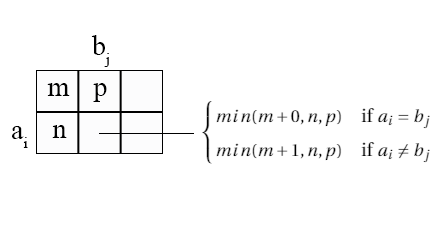
\includegraphics[width=0.7\columnwidth]{books/artificial-neural-network/chapter07/figure-sec4/levdis.png}
		\centering
	\caption{Cách tính khoảng cách Levenshtein.}
	\label{fig:levdis}
\end{figure}

Ví dụ: Khoảng cách Levenshtein giữa \textit{"kitten"} và \textit{"sitting"} là 3 (bảng \ref{Tab:kitten-sitting}), vì phải dùng ít nhất ba lần biến đổi:
\begin{enumerate}
    \item \textit{kitten} -> \textit{sitten} (thay \textit{"k"} bằng \textit{"s"}).
    \item \textit{sitten} -> \textit{sittin} (thay \textit{"e"} bằng \textit{"i"}).
    \item \textit{sittin} -> \textit{sitting} (thêm ký tự \textit{"g"}).
\end{enumerate}

\begin{table}[H]
\caption{Khoảng cách giữa \textit{"kitten"} và \textit{"sitting"}.}
\centering
    \begin{tabular}{|l|l|l|l|l|l|l|l|l|}
    \hline
     &  & \textbf{s} & \textbf{i} & \textbf{t} & \textbf{t} & \textbf{i} & \textbf{n} & \textbf{g} \\ \hline
     & \textbf{0} & \textbf{1} & \textbf{2} & \textbf{3} & \textbf{4} & \textbf{5} & \textbf{6} & \textbf{7} \\ \hline
    \textbf{k} & \textbf{1} & 1 & 2 & 3 & 4 & 5 & 6 & 7 \\ \hline
    \textbf{i} & \textbf{2} & 2 & 1 & 2 & 3 & 4 & 5 & 6 \\ \hline
    \textbf{t} & \textbf{3} & 3 & 2 & 1 & 2 & 3 & 4 & 5 \\ \hline
    \textbf{t} & \textbf{4} & 4 & 3 & 2 & 1 & 2 & 3 & 4 \\ \hline
    \textbf{e} & \textbf{5} & 5 & 4 & 3 & 2 & 2 & 3 & 4 \\ \hline
    \textbf{n} & \textbf{6} & 6 & 5 & 4 & 3 & 3 & 2 & {\color[HTML]{FE0000} \textbf{3}} \\ \hline
    \end{tabular}
    \label{Tab:kitten-sitting}
\end{table}

Áp dụng khoảng cách Levenshtein vào tính khoảng cách phát âm giữa \textit{"pair"} (pe-a) với \textit{"pear"} (pe-a) (bảng \ref{Tab:pear-pair}) và \textit{"strawberry"} (stro-be-ri) (bảng \ref{Tab:strawberry-pair}).
\begin{table}[H]
\caption{Khoảng cách phát âm giữa \textit{"pear"} (pe-a) và \textit{"pair"} (pe-a).}
\centering
    \begin{tabular}{|l|l|l|l|l|}
    \hline
     & & \textbf{p} & \textbf{e} & \textbf{a} \\ \hline
     & \textbf{0} & \textbf{1} & \textbf{2} & \textbf{3} \\ \hline
    \textbf{p} & \textbf{1} & 0 & 1 & 2 \\ \hline
    \textbf{e} & \textbf{2} & 1 & 0 & 1 \\ \hline
    \textbf{a} & \textbf{3} & 2 & 1 & {\color[HTML]{FE0000} \textbf{0}} \\ \hline
    \end{tabular}
    \label{Tab:pear-pair}
\end{table}

\begin{table}[H]
\caption{Khoảng cách phát âm giữa \textit{"strawberry"} (stro-be-ri) và \textit{"pair"} (pe-a).}
\centering
    \begin{tabular}{|l|l|l|l|l|}
    \hline
     &  & \textbf{p} & \textbf{e} & \textbf{a} \\ \hline
     & \textbf{0} & \textbf{1} & \textbf{2} & \textbf{3} \\ \hline
    \textbf{s} & \textbf{1} & 1 & 2 & 3 \\ \hline
    \textbf{t} & \textbf{2} & 2 & 2 & 3 \\ \hline
    \textbf{r} & \textbf{3} & 3 & 3 & 3 \\ \hline
    \textbf{o} & \textbf{4} & 4 & 4 & 4 \\ \hline
    \textbf{b} & \textbf{5} & 5 & 5 & 5 \\ \hline
    \textbf{e} & \textbf{6} & 6 & 5 & 6 \\ \hline
    \textbf{r} & \textbf{7} & 7 & 6 & 6 \\ \hline
    \textbf{i} & \textbf{8} & 8 & 7 & {\color[HTML]{FE0000} \textbf{7}} \\ \hline
    \end{tabular}
    \label{Tab:strawberry-pair}
\end{table}

Ta có thể thấy khoảng cách phát âm giữa \textit{"pear"} (pe-a) và \textit{"pair"} (pe-a) là 0 và giữa \textit{"strawberry"} (stro-be-ri) và \textit{"pair"} (pe-a) là 7, vì thế mô hình sẽ chọn \textit{"pear"} là từ thay thế.

\subsection{Đối với bài toán Image to Text}
Đối với bài toán Image to Text  thì ta phải ưu tiên những từ có đặc điểm, nét viết gần giống với từ sai. Và tất nhiên là những từ đó vẫn phải có xác suất xuất hiện cao.

Ví dụ:
\begin{itemize}
    \item Nhầm lẫn giữa \textit{"1"} và \textit{"4"} (hình \ref{fig:onefour}).
\end{itemize}
% \usepackage{subfig}
\begin{figure}[H]
    \centering
    \subfloat[1]{{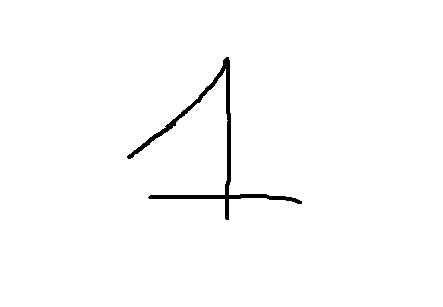
\includegraphics[width=0.3\columnwidth]{books/artificial-neural-network/chapter07/figure-sec4/1.png} }}%
    \qquad
    \subfloat[4]{{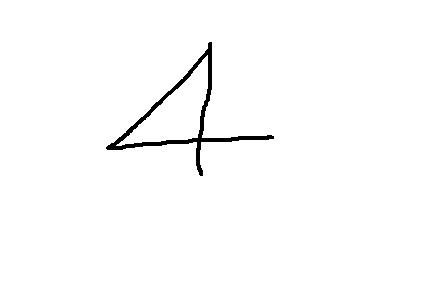
\includegraphics[width=0.3\columnwidth]{books/artificial-neural-network/chapter07/figure-sec4/4.png} }}%
    \caption{Số 1 và số 4 viết tay có nét tương đồng nhau.}%
    \label{fig:onefour}
\end{figure}

\begin{itemize}
    \item Nhầm lẫn giữa \textit{"9"}, \textit{"g"} và \textit{"q"} (hình \ref{fig:ninegq}).
\end{itemize}
\begin{figure}[H]
	\centering
		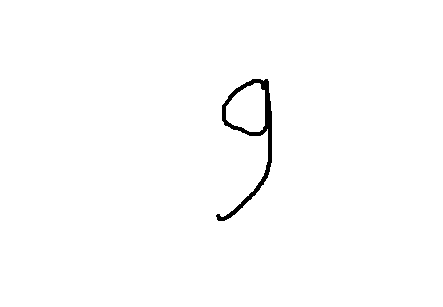
\includegraphics[width=0.5\columnwidth]{books/artificial-neural-network/chapter07/figure-sec4/9-g-q.png}
		\centering
	\caption{Số 9, ký tự g và ký tự q viết tay có nét tương đồng nhau.}
	\label{fig:ninegq}
\end{figure}

Về lĩnh vực này thì chúng ta cũng có thể xây dựng mô hình đánh giá sự tương đồng về nét, hình ảnh của các từ, ký tự. Hoặc chúng ta có thể tạo ra danh sách các ký tự có nét giống nhau và dùng những tập hợp đó để đánh giá và chọn từ sửa lỗi. Ngoài ra còn có thể sử dụng mô hình biến đổi từ (Edit Model) (phần \ref{subsec3}) hoặc tính \textit{Khoảng cách Levenshtein} (công thức \ref{chp7-sec4:eq21}) để chọn từ thay thế, tuy nhiên những cách này không mang nhiều ý nghĩa về sự tương đồng hình ảnh của các ký tự.

Xét ví dụ sau: Nhận diện text trên hình khi sử dụng font chữ dễ gây nhầm lẫn (Bookman Old Style) (hình \ref{fig:bookmanoldstyle}).
\begin{figure}[H]
	\centering
		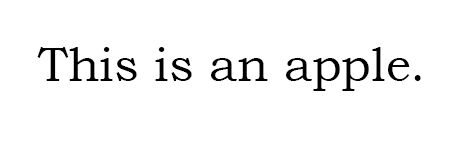
\includegraphics[width=0.5\columnwidth]{books/artificial-neural-network/chapter07/figure-sec4/bookman old style.png}
		\centering
	\caption{Font chữ Bookman Old Style gây nhầm lẫn ký tự \textit{"l"} và số \textit{"1"}.}
	\label{fig:bookmanoldstyle}
\end{figure}

\begin{itemize}
    \item Mô hình dự đoán:
    \begin{center}
    This is an app1e.
    \end{center}
    \item Câu đúng:
    \begin{center}
    This is an apple.
    \end{center}
\end{itemize}

Xác suất khi tính đến từ \textit{"app1e"} sẽ rất thấp hoặc có thể bằng 0, vậy nên mô hình sẽ nghi ngờ đó là từ sai và sẽ tìm từ thay thế.

Mô hình có thể sử dụng các tập hợp các ký tự tương tự nhau để thay vào từ sai và tạo ra tập hợp các ứng cử viên từ đúng và tính xác suất.

Ví dụ:
\begin{itemize}
    \item Tập hợp các ký tự giống số \textit{"1"}: \{1, l, I, i, t, /, |\}
    \item Tập hợp các ứng cử viên sau khi thay thế số \textit{"1"} vào từ sai \textit{"app1e"}: \{apple, appIe, appie, appte, app/e, app|e\}
\end{itemize}

Mô hình sẽ tính được xác suất của từ \textit{"apple"} là cao nhất nên sẽ chọn \textit{"apple"} là từ dùng để sửa lỗi.

\subsubsection{Đối với bài toán sửa lỗi chính tả (typo/spelling)} \label{subsec3}
Đối với bài toán chỉnh sửa lỗi chính tả (typo/spelling), thì ta phải ưu tiên những từ có khoảng cách chính tả gần với từ sai.

Đối với lĩnh vực này, chúng ta có thể xây dựng một số phương pháp như sau:
\begin{itemize}
    \item Dựa trên thống kê lỗi trên dữ liệu văn bản thu thập được để xây dựng mô hình xác xuất. Phương pháp này rất khó thực hiện, vì tần suất lỗi chính tả trong dữ liệu thu thập thường rất thấp. Để có mô hình tốt, cần phải có dữ liệu rất lớn.
    \item Định nghĩa các loại lỗi thường xảy ra và xây dựng mô hình đánh giá khả năng xảy ra lỗi (Edit Model) [\ref{refer:25}]. Đây là phương pháp đơn giản và cũng thường được dùng nhất.
\end{itemize}

Với phương pháp xây dựng mô hình đánh giá khả năng xảy ra lỗi của từ, chúng ta có thể xét tới các loại lỗi chính tả khi nhập từ bàn phím như sau (ví dụ với lỗi xảy ra đối với từ \textit{"example"}):
\begin{itemize}
    \item Lỗi nhập sai ký tự trong từ bằng ký tự khác (replace): e\textbf{x}ample -> e\textbf{z}ample
    \item Lỗi nhập sai thứ tự các ký tự trong từ (transpose): examp\textbf{le} -> exmap\textbf{el}
    \item Lỗi nhập thiếu ký tự trong từ (delete): examp\textbf{l}e -> exampe
    \item Lỗi nhập thừa ký tự (insert): example -> exa\textbf{a}mple
\end{itemize}

Đối với mô hình sửa lỗi này, khi đã phát hiện từ sai từ mô hình ngôn ngữ, ta sẽ áp dụng cả bốn phép biến đổi sau vào từ sai như sau:
\begin{itemize}
    \item Replace: Thay thế mỗi ký tự trong bảng chữ cái vào từng vị trí của từ sai.
    \item Transpose: Đảo từng cặp ký tự liền kề nhau trong từ.
    \item Delete: Xóa từng ký tự trong từ.
    \item Insert: Thêm từng ký tự trong bảng chữ cái vào giữa từng vị trí của từ.
\end{itemize}

Xét ví dụ:
\begin{itemize}
    \item Người dùng nhập vào:
    \begin{center}
    I need an \textit{exampe} for this problem.
    \end{center}
    \item Câu đúng:
    \begin{center}
    I need an \textit{example} for this problem.
    \end{center}
\end{itemize}

Sau khi tính xác suất đến từ \textit{"exampe"} của câu sai, mô hình sẽ tính được xác suất đó là rất thấp hoặc có thể bằng 0 và sẽ nghi ngờ \textit{"exampe"} là từ sai. Sau đó áp dụng mô hình sửa lỗi từ vào từ \textit{"exampe"} để tìm tập các ứng cử viên thay thế như sau:
\begin{itemize}
    \item Replace -> \textbf{a}xampe, \textbf{b}xampe, ..., e\textbf{a}ampe, e\textbf{b}ampe, ..., examp\textbf{y}, examp\textbf{z}
    \item Transpose -> \textbf{xe}ampe, e\textbf{ax}mpe, ex\textbf{ma}pe, exa\textbf{pm}e, exam\textbf{ep}
    \item Delete -> xampe (\textbf{\_xampe}), eampe (\textbf{e\_ampe}), exmpe (\textbf{ex\_mpe}), exape (\textbf{exa\_pe}), exame (\textbf{exam\_e}), examp (\textbf{examp\_})
    \item Insert -> \textbf{a}exampe, \textbf{b}exampe, ..., e\textbf{a}xampe, e\textbf{b}xampe, ..., \underline{examp\textbf{l}e}, examp\textbf{m}e, ..., exampe\textbf{y}, exampe\textbf{z}
\end{itemize}

Sau khi biến đổi như trên, ta sẽ có một tập hợp tất cả các từ đã được biến đổi, từ được chọn để sửa sai sẽ là một từ trong tập hợp trên và có xác suất xuất hiện cao nhất trong bộ dữ liệu. Trong ví dụ trên, từ \textit{"example"} sẽ là từ có xác suất xuất hiện cao nhất nên mô hình sẽ lựa chọn \textit{"example"} là từ được dùng để sửa lỗi.

Phương pháp biến đổi nêu trên để áp dụng cho trường hợp một ký tự lỗi, ta có thể áp dụng tương tự cho các trường hợp nhiều ký tự lỗi, tuy nhiên số lượng từ để xét tới sẽ trở nên lớn, tốc độ xử lý khi sửa lỗi chậm và tập hợp ứng cử viên sẽ lớn nên xác suất nhầm lẫn giữa các từ gần giống nhau về mặt ký tự sẽ lớn.

Ngoài ra, chúng ta có thể tìm tập ứng cử viên trong bộ dữ liệu và sử dụng \textit{Khoảng cách Levenshtein} (công thức \ref{chp7-sec4:eq21}) để tính khoảng cách từ vựng với từ sai và tìm từ thay thế.
